\documentclass[12pt,twoside=false,a4paper,parskip]{scrbook}
% use the following line instead of the class above if you want double-sided printing
% don't remove openright as it looks better in case of double-sided print
% \documentclass{scrbook} 
\usepackage{inputenc}
\usepackage{csquotes}
\usepackage{babel}
\usepackage{floatflt}
\usepackage{float}
\usepackage{subfigure}
\usepackage{graphicx}
\usepackage{hyperref}
\usepackage{color}
\usepackage{amssymb}
\usepackage{textcomp}
\usepackage{nicefrac}
\usepackage{scrhack}
\usepackage{pdfpages}
\usepackage{tabularx}
\usepackage{float}
\usepackage{pdflscape}
\usepackage{subfigure}
\usepackage{pdfpages}
\usepackage{placeins}
\usepackage{scrlayer-scrpage}
\usepackage{listings}
\usepackage{xcolor}
\usepackage{color}
\usepackage{caption}
\usepackage{subfigure}
\usepackage{tocloft}
\usepackage{epstopdf}
\usepackage{longtable}
\usepackage{setspace}
\usepackage{booktabs}
\usepackage{biblatex}
\bibliography{literatur}
\usepackage{hyphenat} % texttt do line breaks
\usepackage{inputenc}
\usepackage{newunicodechar}
\newunicodechar{ }{\,}


\usepackage{amsmath}
\usepackage{amsfonts}
\usepackage{amssymb}
\usepackage{graphicx}
\usepackage{float}
\usepackage{hyperref}
\hypersetup{
colorlinks=true,
linkcolor=blue,
filecolor=magenta,
urlcolor=cyan,
}
\usepackage{enumitem} % Für benutzerdefinierte Listenetiketten
\usepackage{geometry} % Zum Verwalten der Seitenränder
\geometry{a4paper, total={170mm,257mm}, left=20mm, top=20mm} % Standard A4 Ränder

\usepackage{fontenc}    % bessere Trennung (z. B. Umlaute)
\usepackage{microtype}      % feine Mikrotypografie (verbessert Umbrüche & Ränder)

\usepackage[utf8]{inputenc}
\usepackage[T1]{fontenc}
\usepackage[ngerman]{babel}
\usepackage{lmodern}

% --- TikZ für Mindmap ---
\usepackage[margin=18]{geometry}
\usepackage{tikz}
\usetikzlibrary{arrows.meta,positioning,calc,fit,backgrounds}
\usepackage{adjustbox} % für max totalsize





\sloppy                    % großzügigere Zeilenumbrüche (vermeidet Overfull hboxes)


%%%%%%%%%%%%%%%%%%%
%% definitions
%%%%%%%%%%%%%%%%%%%
\def\BaAuthor{Noah Raupold (5022097),\\ David Gläsle(5022114)}
\def\BaAuthorStudyProgram{Informatik} %% Wirtschaftsinformatik, E-Commerce, Informationssysteme
\def\BaType{ADT Portfolio} %% Masterarbeit
\def\BaTitle{Modellierung des Lobbyregisters}
\def\BaDeadline{\today}

\def\iswithfullname{1} % uncomment this to create non-anonymous version
\ifdefined\iswithfullname
\def\ShowBaAuthor{\BaAuthor}
\else
\def\ShowBaAuthor{N.~N.}
\fi

\hypersetup{
pdfauthor={\ShowBaAuthor},
pdftitle={\BaTitle},
pdfsubject={Subject},
pdfkeywords={Keywords}
}

%%%%%%%%%%%%%%%%%%%
%% configs to include
%%%%%%%%%%%%%%%%%%%
\colorlet{punct}{red!60!black}
\definecolor{background}{HTML}{EEEEEE}
\definecolor{delim}{RGB}{20,105,176}
\colorlet{numb}{magenta!60!black}

\definecolor{gray}{rgb}{0.4,0.4,0.4}
\definecolor{darkblue}{rgb}{0.0,0.0,0.6}
\definecolor{cyan}{rgb}{0.0,0.6,0.6}

\definecolor{pblue}{rgb}{0.13,0.13,1}
\definecolor{pgreen}{rgb}{0,0.5,0}
\definecolor{pred}{rgb}{0.9,0,0}
\definecolor{pgrey}{rgb}{0.46,0.45,0.48}

\lstset{
basicstyle=\ttfamily,
columns=fullflexible,
showstringspaces=false,
commentstyle=\color{gray}\upshape
linewidth=\textwidth
}

\lstdefinelanguage{json}{
basicstyle=\normalfont\ttfamily,
numbers=left,
numberstyle=\scriptsize,
stepnumber=1,
numbersep=8pt,
showstringspaces=false,
breaklines=true,
backgroundcolor=\color{background},
literate=
*{0}{{{\color{numb}0}}}{1}
{1}{{{\color{numb}1}}}{1}
{2}{{{\color{numb}2}}}{1}
{3}{{{\color{numb}3}}}{1}
{4}{{{\color{numb}4}}}{1}
{5}{{{\color{numb}5}}}{1}
{6}{{{\color{numb}6}}}{1}
{7}{{{\color{numb}7}}}{1}
{8}{{{\color{numb}8}}}{1}
{9}{{{\color{numb}9}}}{1}
{:}{{{\color{punct}{:}}}}{1}
{,}{{{\color{punct}{,}}}}{1}
{\{}{{{\color{delim}{\{}}}}{1}
{\}}{{{\color{delim}{\}}}}}{1}
{}{{{\color{delim}{]}}}}{1},
}

\lstset{language=xml,
morestring=",
morestring={>}{<},
morecomment={<?}{?>},
stringstyle=\color{black},
numbers=left,
numberstyle=\scriptsize,
stepnumber=1,
numbersep=8pt,
identifierstyle=\color{darkblue},
keywordstyle=\color{cyan},
backgroundcolor=\color{background},
morekeywords={xmlns,version,type}% list your attributes here
}

\lstset{language=Java,
showspaces=false,
showtabs=false,
tabsize=4,
breaklines=true,
keepspaces=true,
numbers=left,
numberstyle=\scriptsize,
stepnumber=1,
numbersep=8pt,
showstringspaces=false,
breakatwhitespace=true,
commentstyle=\color{pgreen},
keywordstyle=\color{pblue},
stringstyle=\color{pred},
basicstyle=\ttfamily,
backgroundcolor=\color{background},
%  moredelim={$$},
%  moredelim={\%\%}{\%\%}
}

\newcommand*{\forcetwosidetitle}{
\begingroup
\cleardoubleoddpage
\KOMAoptions{titlepage=true}% useful e.g. for scrartcl
\csname @twosidetrue\endcsname
\maketitle
\endgroup
}

\newcommand{\TOCbreak}{\\}




\begin{document}

%%%%%%%%%%%%%%%%%%%
%% Titelseite
%%%%%%%%%%%%%%%%%%%
\frontmatter
\titlehead{
{Technische Hochschule Würzburg-Schweinfurt\\
Fakultät Informatik und Wirtschaftsinformatik}}
\subject{\BaType}
\title{\BaTitle\\[15mm]
\begin{figure}[H]
\centering
\includegraphics[width=0.5\textwidth]{Logo.png}
\label{fig:logo}
\end{figure}}
%\subtitle{\normalsize{vorgelegt an der Technischen Hochschule W\"{u}rzburg-Schweinfurt in der Fakult\"{a}t Informatik und Wirtschaftsinformatik zum Abschluss eines Studiums im Studiengang \BaAuthorStudyProgram}}
\author{\ShowBaAuthor}
\date{\normalsize{Eingereicht am: \BaDeadline}}
\forcetwosidetitle
%%%%%%%%%%%%%%%%%%%
%% abstract
%%%%%%%%%%%%%%%%%%%


%%%%%%%%%%%%%%%%%%%
%% Inhaltsverzeichnis
%%%%%%%%%%%%%%%%%%%
\newpage
\setcounter{secnumdepth}{4}
\setcounter{tocdepth}{4}
\tableofcontents



%%%%%%%%%%%%%%%%%%%
%% Main part of the thesis
%%%%%%%%%%%%%%%%%%%
\mainmatter
\mainmatter

\chapter{Einleitung}
Im Rahmen des FWPMs Advanced Database Techniques besteht unsere Aufgabe darin, ein realistisches Anwendungsszenario in ein funktionales Datenbankmodell zu überführen. Als Zielszenario wählten wir die Modellierung des bundesdeutschen Lobbyregisters, mit dem Ziel, die Struktur und Dynamik der Interessenvertretung in Deutschland möglichst präzise und nachvollziehbar abzubilden. Dieses Thema wurde aufgrund seiner hohen gesellschaftlichen Relevanz sowie der vielfältigen, strukturiert erfassbaren Datenaspekte ausgewählt.

Das Lobbyregister bietet eine komplexe Datenlandschaft aus Organisationen, Einzelpersonen, Tätigkeitsbereichen und Finanzflüssen, die gemeinsam ein transparentes Bild politischer Einflussnahme ermöglichen sollen. Neben den grundlegenden Entitäten wie Interessenvertreterinnen und -vertreter, Mandatsträgern und Organisationen liegt ein besonderer Schwerpunkt auf der Modellierung von Beziehungen und Aktivitäten, um Zusammenhänge und Netzwerke im Bereich der Interessenvertretung sichtbar zu machen.

Darüber hinaus stellt die Integration halbstrukturierter Daten – etwa in Form von JSON-Dokumenten oder erläuternden Textfeldern – eine besondere Herausforderung dar, die wir mit Blick auf Flexibilität und Erweiterbarkeit gezielt adressieren. Durch die Wahl von PostgreSQL als zugrunde liegender Datenbanktechnologie können sowohl relationale als auch semi-strukturierte Daten effizient verwaltet und analysiert werden.

Der Fokus dieses ersten Portfolioteils lag auf der konzeptionellen Modellierung. Im Folgenden stellen wir unseren Ansatz bei der Ideenfindung, der Definition relevanter Entitäten und Beziehungen sowie der Erstellung des Entity-Relationship-Modells (ERM) vor. Abschließend reflektieren wir die bisherigen Erkenntnisse und begründen die Entscheidung für die eingesetzte Datenbanktechnologie.

\chapter{Ideensammlung}
Zu Beginn haben wir in einer gemeinsamen Diskussionsrunde verschiedene Anwendungsszenarien abgewogen. Dabei war uns wichtig:

\begin{itemize}
\item Ein Szenario mit realem gesellschaftlichem Bezug.
\item Ein Datensatz, der sowohl Stammdaten (Organisationen, Personen) als auch Bewegungsdaten (Lobbyaktivitäten, Treffen, Finanzen) enthält.
\item Ein Umfeld, in dem wir die Vorteile einer relationalen Datenbank nutzen können – also mit vielen Relationen, Fremdschlüsselbeziehungen und ggf. halb-strukturierten Daten.
\end{itemize}

Das Thema „Lobbyregister“ überzeugte uns insbesondere, weil:

\begin{itemize}
\item In Deutschland mit dem Lobbyregister der Bundestagsverwaltung erstmals ein zentrales Register für Interessenvertretung vorliegt.
\item Es zahlreiche Entitäten gibt: Lobbyorganisationen, Lobbyagenturen, Auftraggeber, Einzelpersonen, Finanzierung, gesetzgebende Prozesse, Ziele, Treffen etc.
\item Es Potenzial für Analyse gibt: z. B. welche Branchen besonders aktiv sind, welche Verbindungen bestehen, wieviel Geld geflossen ist, welche Gesetzesinitiativen betroffen sind.
\item Es auch Möglichkeiten für Datenimport und -integration gibt, z. B. Öffentliche Daten, APIs oder CSV/JSON-Quellen.
\end{itemize}

Wir haben eine Mindmap erstellt, in der wir zentrale Elemente des Registers identifizierten, etwa:

\begin{itemize}
\item Lobbyorganisationen (Name, Rechtsform, Sitz, Branche)
\item Auftraggeber und Auftragnehmer von Lobbyarbeit
\item Einzelpersonen (Lobbyistinnen und Lobbyisten)

\item Finanzinformationen: Budget, Ausgaben, Drittfinanzierung
\item Interessen- bzw. Zielkatalog: Welche Themen verfolgt die Lobbyarbeit?
\end{itemize}

Auf dieser Grundlage haben wir uns entschieden, die Datenbank so zu entwerfen, dass sie sowohl relationale Struktur (z. B. Organisationen Personen Lobbytätigkeit) abbildet, als auch flexible Datenformate unterstützen kann (z. B. JSON-Struktur für Dokumente oder Erklärungen).
% Beispiel: jede Seite eine runde Mindmap
\section*{Registereintrag}


\begin{figure}[h]
\centering
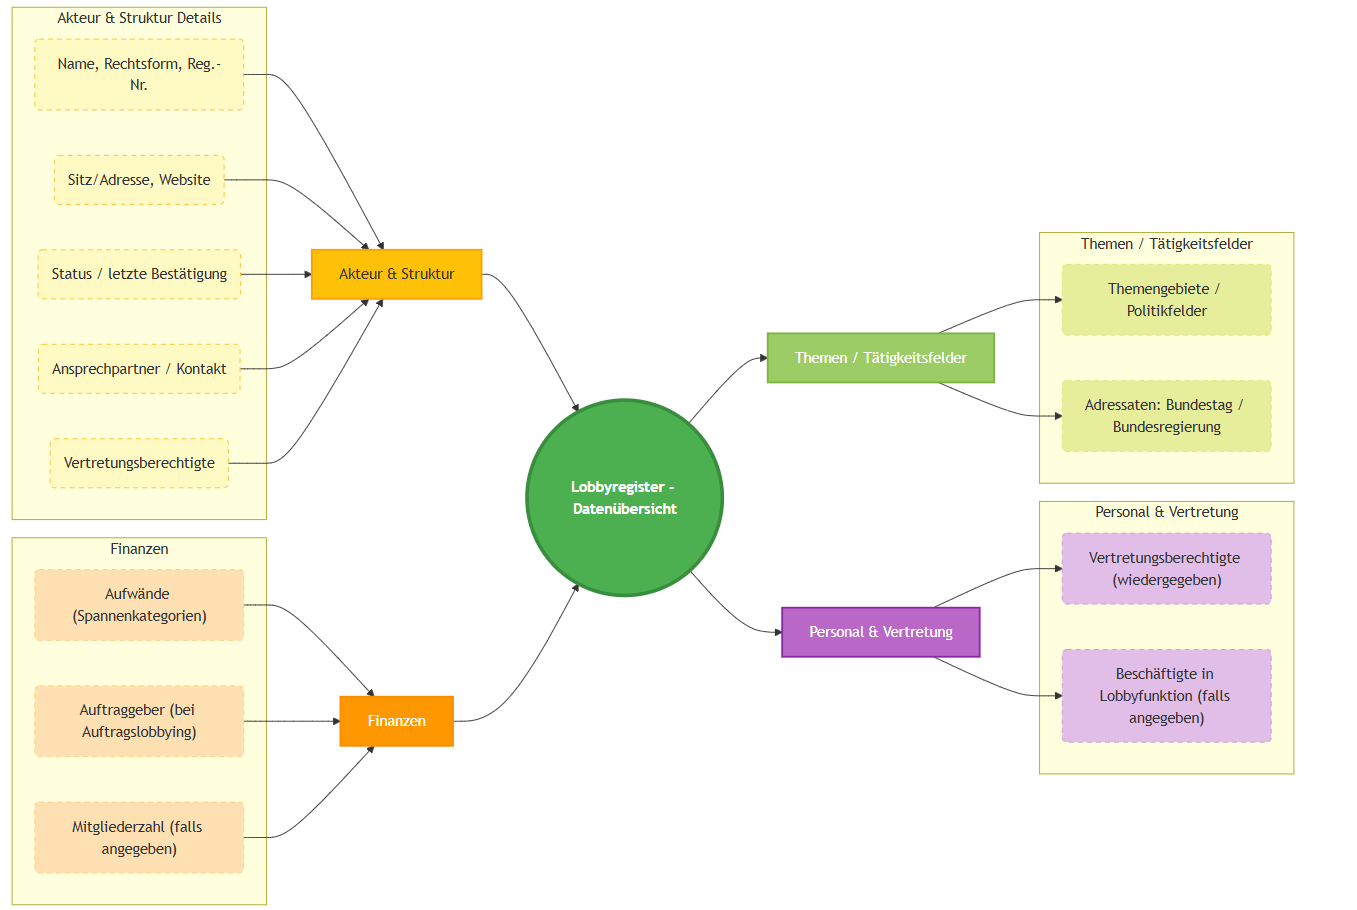
\includegraphics[width=1\textwidth]{overview.png} % Replace with your file name
\caption{Ein Auschnitt des Registereintrages}
\label{fig:example}
\end{figure}


\newpage


\chapter{Use-Case: Analyse von Lobbyaktivitäten}
Das gewählte Szenario eröffnet verschiedene spannende Use-Cases. Beispiele:

\begin{itemize}
\item Analyse, welche Branchen (z. B. Automobil, Energie, Versicherungen) die höchsten Ausgaben für Lobbying haben.
\item Untersuchung von Verbindungen zwischen Lobbyist*innen und Wechsel in öffentliche Ämter („Revolving Door“) – welche Einzelpersonen arbeiten vorher für Verbände und später im öffentlichen Dienst oder umgekehrt.
\item Darstellung von Gesetzesvorhaben und dazugehörigen Lobbyaktivitäten – z. B. welche Organisationen sich zu einem bestimmten Gesetzesentwurf gemeldet haben, mit welchem Ziel und mit welchem Budget.
\item Zeitliche Analyse: Wie verändert sich die Lobbying-Aktivität über Zeit (Jahre, Wahlperioden)?
\end{itemize}

Diese Use-Cases zeigen, dass wir nicht nur eine statische Datenstruktur erstellen, sondern auch Abfragen, Auswertungen und Reports ermöglichen wollen – was Anforderungen an das Datenbankmodell und an das DBMS stellt.

\chapter{Datenmodell}
\label{ch:datamodell}

Dieses Kapitel beschreibt das zentrale Datenmodell, das zur Abbildung der Informationen aus dem Lobbyregister des Deutschen Bundestages über die bereitgestellte API dient.

Um die tief verschachtelten JSON-Daten der API in einer performanten und konsistenten relationalen Datenbank (PostgreSQL) zu speichern, wurde ein vollständig normalisiertes Schema in der 3. Normalform (3NF) entworfen. Das resultierende physische Datenmodell ist sehr detailliert und besteht aus **insgesamt 84 einzelnen Tabellen**. Diese hohe Anzahl entsteht durch die konsequente Auflösung aller Listen (Arrays), wiederverwendbarer Strukturen (wie Adressen oder Codelisten) und verschachtelter Objekte in eigene Tabellen, die über Fremdschlüssel miteinander verbunden sind.

Eine vollständige Dokumentation aller 84 Tabellen würde den Rahmen dieser Arbeit sprengen. Dieses Kapitel beschreibt daher als repräsentativen **Ausschnitt** die konzeptionelle Grundlage dieses Schemas. Es konzentriert sich auf die beiden Hauptentitäten, wie sie von der API definiert werden: \texttt{RegisterEntry} und \texttt{RegisterEntryStatistics}. Diese bilden den logischen Ausgangspunkt, aus dem das normalisierte 84-Tabellen-Schema abgeleitet wurde.

Die Basis-URL für die API-Aufrufe ist \texttt{https://api.lobbyregister.bundestag.de/rest/v2} .

\section{Hauptentität: RegisterEntry}

Die Entität \texttt{RegisterEntry} stellt einen vollständigen Registereintrag dar  und ist die zentrale Ressource, die über die Endpunkte wie \texttt{/registerentries/\{registerNumber\}} abgerufen werden kann .

Die Entität beinhaltet die folgenden Hauptkomponenten:
\begin{itemize}
\item \texttt{source}, \texttt{sourceUrl}, \texttt{sourceDate}, \texttt{jsonDocumentationUrl}: Metadaten zur Quelle und zum Zeitpunkt der Datenabfrage.
\item \texttt{registerNumber}: Die eindeutige Registernummer des Eintrags, deren Format dem Muster \verb|^R\d{6}$| folgt (z.\,B. R001234).
\item \texttt{accountDetails}: Enthält Informationen zum Zustand des Kontos der Interessenvertretung (IV) .
\item \texttt{registerEntryDetails}: Detaillierte, versionsspezifische Informationen zum Eintrag .
\item \texttt{lobbyistIdentity}: Informationen zur Identität der Interessenvertreterin/des Interessenvertreters .
\item \texttt{activitiesAndInterests}: Informationen zu Tätigkeiten und Interessenbereichen .
\item \texttt{clientIdentity}: Angaben zur Identität des Auftraggebers/der Auftraggeberin, falls vorhanden .
\item \texttt{employeesInvolvedInLobbying}: Angaben zu den im Bereich der Interessenvertretung beschäftigten Personen .
\item \texttt{financialExpenses}: Angaben zu den jährlichen finanziellen Aufwendungen für Interessenvertretung .
\item \texttt{publicAllowances}: Angaben zu Zuwendungen und Zuschüssen .
\item \texttt{donators}: Angaben zu Schenkungen .
\item \texttt{membershipFees}: Angaben zu Mitgliedsbeiträgen .
\item \texttt{annualReports}: Angaben zum Jahresabschluss/Rechenschaftsbericht .
\item \texttt{regulatoryProjects}: Angaben zu Regelungsvorhaben, zu denen Interessenvertretung betrieben wird .
\item \texttt{statements}: Angaben zu Stellungnahmen/Gutachten .
\item \texttt{contracts}: Angaben zu Aufträgen für Interessenvertretung .
\item \texttt{codeOfConduct}: Angaben zum Verhaltenskodex .
\end{itemize}

\subsection{Detaillierte Sub-Entitäten von RegisterEntry}

\subsubsection{AccountDetails}
Diese Struktur enthält Zustandsinformationen des Kontos :
\begin{itemize}
\item \texttt{activeLobbyist}: Gibt an, ob die IV aktuell aktive (TRUE) oder inaktive (FALSE) Interessenvertretung betreibt .
\item \texttt{registerEntryVersions}: Eine Liste (\texttt{array}) aller Versionen, die für das Konto vorliegen . Jede Version enthält die interne ID (\texttt{registerEntryId}), die Versionsnummer (\texttt{version}), die zugrundeliegende Gesetzeslage (\texttt{legislation}, z.B. GL2022 oder GL2024), und den Gültigkeitszeitraum (\texttt{validFromDate}, \texttt{validUntilDate}) .
\item \texttt{accountHasCodexViolations}: Wahr, wenn mindestens ein Verstoß gegen den Verhaltenskodex vorliegt .
\item \texttt{codexViolations}: Liste der aktiven Verstöße gegen den Verhaltenskodex, mit dem Attribut \texttt{codexViolationName} .
\end{itemize}

\subsubsection{LobbyistIdentity}
Diese Struktur beschreibt die Identität des Interessenvertreters/der Interessenvertreterin :
\begin{itemize}
\item \texttt{identity}: Personentyp der IV, entweder \texttt{NATURAL} (natürliche Person) oder \texttt{ORGANIZATION} (Organisation) .
\item Natürliche Personen nutzen Attribute wie \texttt{lastName}, \texttt{firstName} (GL2024), \texttt{commonFirstName} (GL2022) und akademische Grade (\texttt{academicDegreeBefore/After}) .
\item Organisationen nutzen \texttt{companyName} , \texttt{legalFormType} und \texttt{legalForm} .
\item Die Struktur enthält ferner Angaben zu Adress- und Kontaktdaten (\texttt{address}, \texttt{contactDetails}) , zur Hauptstadtrepräsentanz (\texttt{capitalCityRepresentation}) , sowie Listen von betrauten Personen (\texttt{entrustedPersons})  und gesetzlichen Vertreter/-innen (\texttt{legalRepresentatives}) .
\end{itemize}

\subsubsection{ActivitiesAndInterests}
Informationen zu den Aktivitäten der Interessenvertretung :
\begin{itemize}
\item \texttt{activity}: Informationen zur Tätigkeit selbst, inklusive \texttt{code}, deutscher (\texttt{de}) und englischer (\texttt{en}) Bezeichnung .
\item \texttt{typesOfExercisingLobbyWork}: Liste der Arten der Ausübung der Interessenvertretung .
\item \texttt{fieldsOfInterest}: Eine Liste der Interessenbereiche .
\item \texttt{activityOperationType}: Gibt an, ob die Interessenvertretung \texttt{SELF\_OPERATED}, \texttt{MANDATE\_OPERATED} oder \texttt{BOTH} betrieben wird .
\item \texttt{legislativeProjects}: Liste der Gesetzesvorhaben, inklusive Name und Drucksachennummer (\texttt{printingNumber}) .
\end{itemize}

\subsubsection{FinancialExpenses}
Angaben zu den jährlichen finanziellen Aufwendungen für Interessenvertretung :
\begin{itemize}
\item \texttt{refuseFinancialExpensesInformation}: Gibt an, ob Angaben verweigert wurden .
\item \texttt{relatedFiscalYearFinished}, \texttt{relatedFiscalYearStart}, \texttt{relatedFiscalYearEnd}: Details zum Bezugsgeschäftsjahr (relevant für GL2024) .
\item \texttt{financialExpensesEuro}: Zahlenbereich (\texttt{from}/\texttt{to}) der jährlichen Aufwendungen in Euro .
\end{itemize}

\subsubsection{RegulatoryProjects}
Angaben zu konkreten Regelungsvorhaben :
\begin{itemize}
\item \texttt{regulatoryProjectsPresent}: Gibt an, ob Interessenvertretung hinsichtlich eines konkreten Regelungsvorhabens betrieben wird .
\item \texttt{regulatoryProjects}: Liste der Regelungsvorhaben, jeweils mit \texttt{regulatoryProjectNumber} (RVxxxxxxx) und \texttt{title} .
\item Enthält Details zu vorhandenen Drucksachen (\texttt{printedMatters})  und Referentenentwürfen (\texttt{draftBill}) .
\end{itemize}

\section{Hilfsentität: RegisterEntryStatistics}

Die Entität \texttt{RegisterEntryStatistics} dient der Bereitstellung von Kennzahlen und Statistiken zu den Registereinträgen .

\begin{itemize}
\item Die Statistikdaten sind im Objekt \texttt{registerEntries} enthalten .
\item \texttt{activeLobbyistsLegalFormType}: Aufteilung der aktiven Interessenvertreter/-innen nach Personentypen, z.B. \texttt{naturalPersons}, \texttt{juristicPersons} und \texttt{legalAssociations} (Personengesellschaften) . Jeder Typ listet \texttt{number} und \texttt{percentage} auf .
\item \texttt{codexViolationOrLateUpdate}: Statistiken zu Verstößen gegen den Verhaltenskodex (\texttt{codexViolation}) oder fehlender Aktualisierung des Geschäftsjahres (\texttt{lateUpdate}) .
\item \texttt{lobbyists}: Gesamtanzahl aller IVs, unterteilt in \texttt{active} und \texttt{inactive} .
\item \texttt{peopleInvolvedInLobbyistWork}: Gesamtanzahl aller Personen, die Interessenvertretung betreiben (IVs und betraute Personen) .
\item \texttt{recentGovernmentFunction}: Statistiken zum "Drehtüreffekt" (\texttt{existing} vs. \texttt{notExisting}), aufgeschlüsselt nach Bundesregierung, Bundestag und Bundesverwaltung .
\item \texttt{fieldsOfInterest}: Listen der Obergruppen (\texttt{mainGroups}) und Untergruppen (\texttt{subgroups}) der Interessenbereiche, jeweils mit Anzahl und prozentualem Anteil .
\item \texttt{activities}: Liste der Tätigkeitskategorien der IVs, ebenfalls mit Anzahl und prozentualem Anteil .
\end{itemize}

\section{Codierte Hilfsobjekte}
Viele Objekte innerhalb der Hauptentitäten verwenden ein standardisiertes Format für Bezeichnungen, die über Codes referenziert werden. Beispiele hierfür sind \texttt{naturalPersonType} , \texttt{country} , \texttt{type} des Drehtüreffekts  oder \texttt{fieldsOfInterest} . Diese Objekte haben typischerweise die Attribute \texttt{code}, \texttt{de} (deutsche Bezeichnung) und \texttt{en} (englische Bezeichnung) .

Nachteile, die wir in Kauf genommen haben:

\begin{itemize}
\item Höhere Einstiegshürde im Vergleich zu einfacheren Systemen.
\item Möglicherweise höherer Ressourcenverbrauch bei großer Last.
\end{itemize}

\chapter{Reflexion / Erkenntnisse}
Zu Beginn standen wir vor Herausforderungen: Definition der Anforderungen, klare Abstimmung innerhalb der Gruppe, Auswahl der richtigen Entitäten und Attribute, Aufbau des Modells. Schnell zeigte sich, dass insbesondere die Modellierung der flexiblen Datenfelder (Themenlisten, Dokumente) sowie die Balance zwischen Normalisierung und Performanz sorgfältig bedacht werden musste.

Positiv war, dass die Wahl von PostgreSQL uns viel Freiraum gab. Wir konnten eine hybride Strategie verfolgen:

\begin{itemize}
\item \textbf{Relationale Normalisierung:} Für klar strukturierte 1:N- oder N:M-Beziehungen (z.B. \texttt{LobbyistIdentity} zu \texttt{LegalRepresentatives} oder die Verknüpfung von \texttt{RegisterEntry} zu \texttt{InterestsTopics}) wurde eine klassische Normalisierung mit Fremdschlüsseln gewählt. Dies ist essenziell für Joins und aggregierte Abfragen.

\item \textbf{Nutzung von JSONB:} Für tief verschachtelte, variable oder selten abgefragte Listen (z.B. die \texttt{expensesBreakdown} innerhalb von \texttt{financialExpenses} oder die Liste der \texttt{statements}) wurde der JSONB-Datentyp genutzt.

\item \textbf{Begründung:} Diese Balance verhindert eine "Schema-Explosion" (potenziell 50+ Tabellen bei voller Normalisierung) und hält die Komplexität beherrschbar, während die relationale Stärke für die Kernanalysen (Use-Cases) erhalten bleibt.
\end{itemize}

Wir haben gelernt, dass die gesellschaftliche Relevanz eines Szenarios (wie das Lobbyregister) die Motivation stärkt und dass eine reale Datenquelle – zumindest als Beispiel – hilfreich ist. Zudem wurde klar: Dokumentation der technischen Entscheidungen (z. B. DBMS-Wechsel) gehört unbedingt ins Portfolio.
\chapter{Fazit}

Den ersten Meilenstein in der Entwicklung unserer Datenbank – die Erstellung eines konzeptionellen Datenmodells – konnten wir als Team erfolgreich abschließen. Dabei zeigte sich jedoch, dass der damit verbundene Aufwand größer war, als wir anfangs angenommen hatten. Besonders die Modellierung der vielfältigen Entitäten und Beziehungen innerhalb des Lobbyregisters erwies sich als komplex, da insbesondere die Balance zwischen struktureller Normalisierung und technischer Flexibilität sorgfältig abgestimmt werden musste.

Herausfordernd war vor allem der Umgang mit variablen und tief verschachtelten Datenstrukturen, wie sie beispielsweise bei Themenlisten oder Finanzangaben auftreten. Die Entscheidung, neben klassischen relationalen Strukturen auch JSONB-Felder einzusetzen, erwies sich dabei als sinnvoller Kompromiss zwischen Performance und Wartbarkeit.

Trotz der anfänglichen Herausforderungen empfanden wir die Arbeit mit PostgreSQL insgesamt als positiv. Die vertraute SQL-Syntax sowie die erweiterten Funktionen für semi-strukturierte Daten ermöglichten es uns, ein robustes und zugleich flexibles Datenmodell zu entwerfen. Besonders hilfreich war zudem die enge Zusammenarbeit im Team, um konzeptionelle und technische Entscheidungen abzustimmen und die Komplexität des Projekts gemeinsam zu bewältigen.

\chapter{Ausblick / Weiteres Vorgehen}

In den kommenden Arbeitsschritten werden wir das entworfene Datenmodell in PostgreSQL umsetzen und auf Basis der definierten Use-Cases weiterentwickeln. Für die Visualisierung der Daten planen wir den Einsatz von Grafana, da es umfangreiche Analysemöglichkeiten sowie eine native Unterstützung für PostgreSQL bietet.

Im Rahmen der Implementierung werden wir gezielt auf Performance-Optimierungen eingehen. So sollen beispielsweise \textbf{Materialized Views} für aggregierte Finanzanalysen erstellt und spezielle Indizes (z. B. \textbf{GIN-Indizes} auf JSONB-Feldern) eingerichtet werden, um komplexe Suchanfragen – etwa nach ehemaligen Regierungsmitgliedern oder finanziellen Verflechtungen – effizient zu gestalten.

Langfristig ist geplant, auf Basis der Datenbank interaktive Auswertungen und Visualisierungen zu realisieren. Denkbar ist etwa der Aufbau eines Dashboards, das zentrale Kennzahlen wie Branchenvergleiche oder Netzwerkstrukturen von Organisationen und Personen darstellt. Zudem könnte das Modell durch automatisierte Datentransformationen erweitert werden, um regelmäßig neue Registerdaten zu integrieren.

Damit legen wir den Grundstein für eine datenbankgestützte Analyse des Lobbyregisters, die sowohl technische als auch gesellschaftliche Aspekte sichtbar macht und zukünftige Erweiterungen – etwa durch Webanwendungen oder API-Anbindungen – ermöglicht.


\backmatter

\end{document}